\section{Modelado}
% Se define la entrada del sistema como la se˜nal de comando u al servomotor. Indique cu´al es la se˜nal de
% comando que utilizar´a para comandar el mismo (sea la real, o sea virtual a conveniencia), cu´ales son los
% valores l´ımites, y cu´al es el concepto f´ısico relacionado a dicho valor.
% Se define la salida como la posici´on del carro p, obtenido del sensor de distancia. Indique c´omo se
% representa dicho valor en el sistema, en qu´e direcci´on est´a definido, cu´ales son los valores l´ımites que considera.
% Se define otra variable como el ´angulo de la barra θ, la cual puede considerarse una variable de estado
% del sistema. Indique c´omo se representa dicho valor en el sistema, en qu´e direcci´on est´a definido, cu´ales son
% los valores l´ımites que considera.
% Obtener una representaci´on en variables de estado, y una transferencia entrada-salida del sistema, lin-
% ealizado en torno al punto donde la barra est´a perfectamente horizontal, y el carro o bola se encuentra en el
% centro de dicha barra, que se denominar´a el punto de equilibrio. El modelo del sistema puede obtenerse de
% cualquier manera conveniente. Puede utilizarse un modelo matem´atico donde se midan de manera directa
% los valores de las variables (pesos, largos, momentos de inercia). Tambi´en un modelo mixto donde se iden-
% tifiquen de manera pr´actica algunos par´ametros o transferencias del sistema. Es posible tambi´en utilizar un
% modelado tipo caja negra. Sin embargo, deben recordarse y tenerse en cuenta las ventajas y sobre todo las
% desventajas de cada uno.

El sistema a modelar se muestra en la Figura~\ref{fig:planta}. Consiste de un servomotor que mueve una barra a través de un brazo. Sobre la barra se coloca un carrito que se desliza libremente. Además, cuenta con una IMU que es capaz de medir el ángulo de la barra, y con un sensor de distancia que mide la posición del carrito a lo largo de la barra.

\begin{figure}[!htbp]
    \centering
    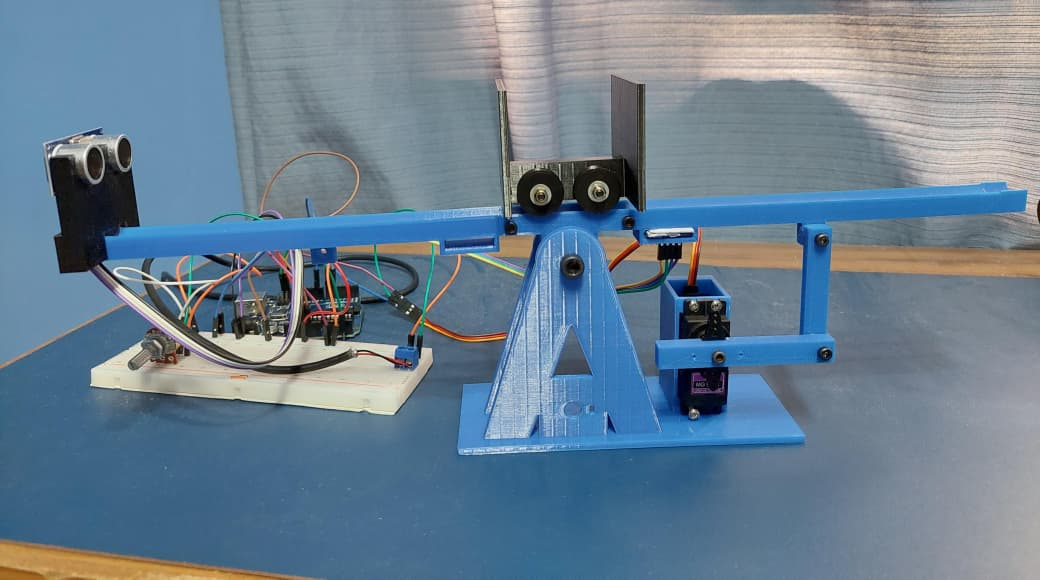
\includegraphics[width=\linewidth]{img/planta.jpg}
    \caption{Sistema \emph{ball-and-beam} a analizar durante el trabajo.}
    \label{fig:planta}
\end{figure}

\subsection{Entrada del sistema}

Para realizar el control de la planta, se define como entrada de la misma el comando $u$ enviado al servomotor, en grados. Se mide positivamente ángulos antihorarios. El comando real del servomotor se realiza a través de la duración de un pulso PWM, donde un valor de \qty{1500}{\us} se corresponde con un \emph{setpoint} de \qty{0}{\degree} respecto de la horizontal. El ángulo comandado al servomotor se mueve linealmente entre \qty{-90}{\degree} para una entrada temporal de \qty{500}{\us}, y \qty{90}{\degree} para \qty{2500}{\us}. Dado que existe una sencilla relación afín entre el tiempo y el ángulo comandado, es válido utilizar el ángulo comandado como entrada virtual dada su mayor interpretabilidad.

Como el ángulo comandado al servomotor se traduce a través del brazo hacia la barra en forma no lineal, solo es conveniente mover el servomotor una cantidad limitada de grados para mantener al sistema alrededor de un punto donde haya una relación aproximadamente lineal entre el ángulo del servo y el de la barra. Por ello, se decidió limitar la entrada al sistema en el rango \qtyrange{-30}{30}{\degree}.

\subsection{Salida del sistema}

Como salida del sistema se considera a la posición $p$ del carro. La misma mide la posición en metros del centro geométrico del carrito, respecto del centro de la barra. La dirección positiva es la que se aleja del sensor de distancia.

Los valores límites de la posición son \qty{-0.152}{\m} y \qty{0.172}{\m}. El extremo inferior se corresponde con la posición más negativa que puede tomar el carrito y aún ser detectado por el sensor de distancia, que es incapaz de medir distancias muy pequeñas. El extremo superior se corresponde con el carro justo en el otro extremo de la barra.

\subsection{Ángulo de la barra}

Otra variable de interés para el modelado del sistema es el ángulo de la barra $\theta$, medido en grados respecto de la horizontal. Este ángulo se mide positivamente en sentido antihorario, tal como el ángulo comandado al servo. Asumiendo la relación linealizada entre estos dos ángulos, donde en estado estacionario $\theta \approx 0.39 u$, los límites de $\theta$ estarán dados por el rango de \qtyrange{-11.7}{11.7}{\degree}.

\subsection{Representación en variables de estado}

El sistema se representará en variables de estado alrededor del punto de equilibrio conformado por la barra en posición horizontal y el carro perfectamente centrado, tal como muestra la Figura~\ref{fig:planta}. Se considera al sistema como la concatenación de dos subsistemas: el sistema servo-barra cuya entrada es el comando al servo $u$ y su salida es el ángulo de la barra $\theta$; y el sistema conformado por el carro, cuya entrada es el ángulo de la barra y su salida es la posición del carro $y = p$.

Entonces, podemos escribir la transferencia completa del sistema como
\[
    \frac{Y(s)}{U(s)} = \frac{\Theta(s)}{U(s)} \frac{Y(s)}{\Theta(s)},
\]
donde la primera transferencia del lado derecho representa la dinámica del sistema servo-barra, y la segunda representa la dinámica del carro en función del ángulo de la barra.

\subsubsection{Sistema servo-barra}

Para obtener la transferencia $\Theta(s) / U(s)$, primero se notó que el sistema consiste de una parte mecánica de un grado de libertad que puede representarse por un sistema de segundo orden, y luego una parte eléctrica dentro del servomotor que es difícil de representar pero tiene una dinámica muy rápida. Por lo tanto, se decidió representar a la transferencia como un sistema de segundo orden con dos polos y ningún cero, quedando de la siguiente forma:
\[
    \frac{\Theta(s)}{U(s)} = \frac{K}{(s+p_1)(s+p_2)}.
\]

Se realizó una identificación del sistema a una frecuencia de \qty{50}{\Hz}, introduciendo como comando al servo escalones simétricos de diferentes amplitudes en grados, y midiendo el ángulo de la barra. El sistema discreto a identificar tiene la forma:
\[
    \frac{\Theta(z)}{U(z)} = \frac{\gamma}{1 - \alpha z^{-1} - \beta z^{-2}}.
\]

\begin{figure}[!htbp]
    \centering
    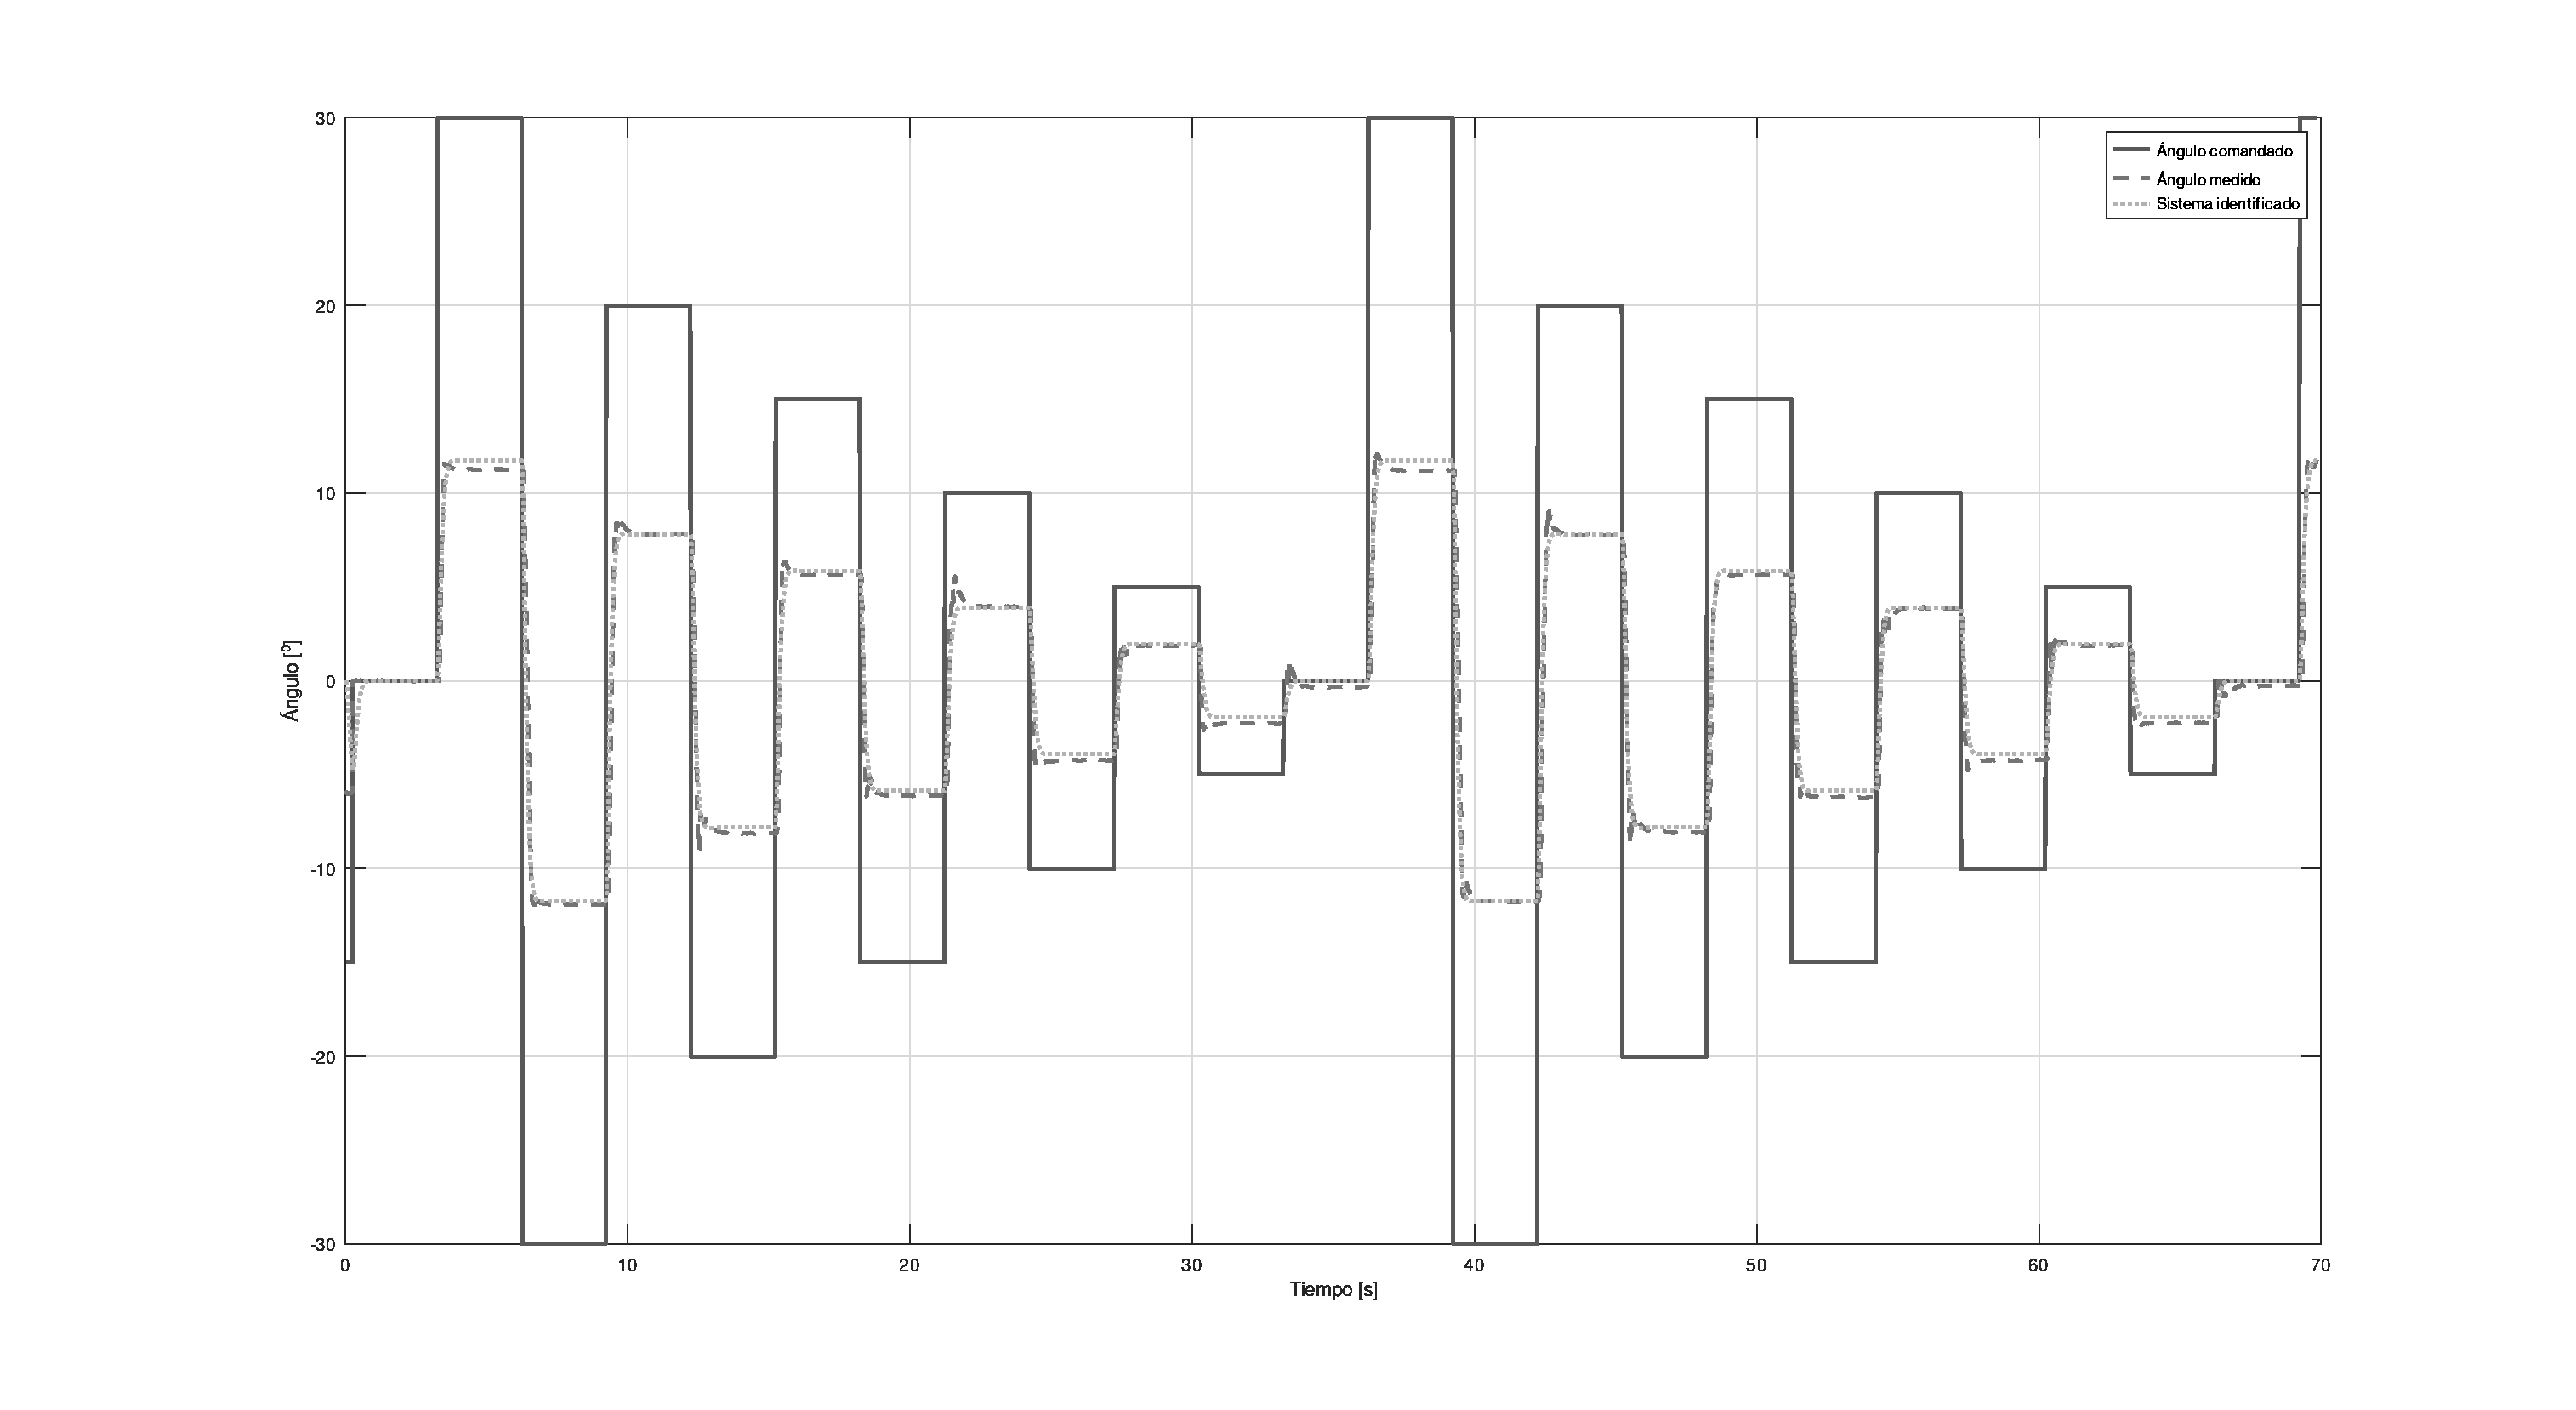
\includegraphics[width=\linewidth]{img/ident-barra.eps}
    \caption{Señales comandada y medida, y salida del sistema servo-barra identificado.}
    \label{fig:ident-barra}
\end{figure}

La Figura~\ref{fig:ident-barra} muestra la señal comandada al servomotor, y el ángulo medido de la barra. Además, se muestra la salida del sistema identificado por regresión lineal. Se observa una buena concordancia entre la salida del sistema real y el identificado. Como resultado de la identificación del sistema se encontró que
\begin{align*}
    \alpha = 1.61 && \beta = -0.652 && \gamma = 0.0174.
\end{align*}
De aquí se pueden despejar los polos discretos, los cuales resultan en
\begin{align*}
    p_{1,2}^{(d)} = 0.804 \pm 0.0775j,
\end{align*}
y utilizando la relación entre polos discretos y continuos dada por
\[
    p^{(d)} = e^{p T_s},
\]
con $T_s = 1/f_s = \qty{20}{\ms}4$, se llega a que los polos del sistema servo-barra son
\begin{align*}
    p_{1,2} = -10.7 \pm 4.81j.
\end{align*}
El sistema entonces es ligeramente oscilante, con una frecuencia de oscilación $w_d = \qty{4.81}{\radian\per\s}$ (aproximadamente \qty{0.8}{\Hz}) y un coeficiente de amortiguamiento $\zeta = 0.91$ (casi críticamente amortiguado). Su transferencia es
\begin{align*}
    \frac{\Theta(s)}{U(s)} = \frac{53.64}{s^2 + 21.4 s + 137.6}
    = \frac{0.39}{\left(\frac{s}{11.73}\right)^2 + 2 \frac{0.91 s}{11.73} + 1}.
\end{align*}

\subsubsection{Sistema barra-carrito}

Para obtener la transferencia entre el ángulo de la barra y la posición del carrito $Y(s) / \Theta(s)$, se considera que el sistema linealizado alrededor del equilibrio (barra horizontal y carro centrado) tiene un polo en cero, y otro polo estable cuya posición depende del momento de inercia de las ruedas, la masa del carro, y la fricción viscosa del sistema. Por lo tanto, en forma simplificada tenemos
\[
    \frac{Y(s)}{\Theta(s)} = \frac{A}{s(s+p)}.
\]
El sistema discreto equivalente tendrá un polo en $z = 1$ proveniente del integrador en el sistema continuo, y otro polo $p^{(d)}$ a determinar, es decir,
\[
    \frac{Y(z)}{\Theta(z)} = \frac{K^{(d)}}{(z-1)(z+p^{(d)})} = \frac{b z^{-2}}{1 + a z^{-1} - (1+a) z^{-2}}
\]

Para realizar el reconocimiento del polo faltante, se agregó un controlador proporcional al sistema con $k_p = 100$. Al sistema realimentado se le aplicaron referencias de posición de $\pm \qty{0.05}{\m}$, y se midió el ángulo de la barra y la posición del carrito. Se realizó una regresión lineal a partir de los datos, donde se halló
\begin{align*}
    a = -0.5386 && b = \num{-5.7326e-04}.
\end{align*}
Esto resulta en un polo discreto $p^{(d)} = -0.4614$, y a través de la relación entre polos discretos y continuos tenemos que el polo continuo está en
\[
    p = -38.7,
\]
de donde la transferencia resulta
\begin{align*}
    \frac{Y(s)}{\Theta(s)} = \frac{-0.7585}{s(s+38.7)}.
\end{align*}
La ganancia puede calcularse como $A = p b/(2+a)/Ts$.

La Figura~\ref{fig:ident-carro} muestra el ángulo medido de la barra, la posición medida del carrito, y la salida del sistema encontrado por regresión. Si bien el sistema identificado presenta una deriva considerable que no se observa en la realidad (debido a la acumulación de errores por la presencia del integrador), la forma de la señal en cortos períodos de tiempo se asemeja a la posición real de carrito para un ángulo dado de la barra. Es decir, se captura correctamente la dinámica del sistema con la identificación hecha.

\begin{figure}[!htbp]
    \centering
    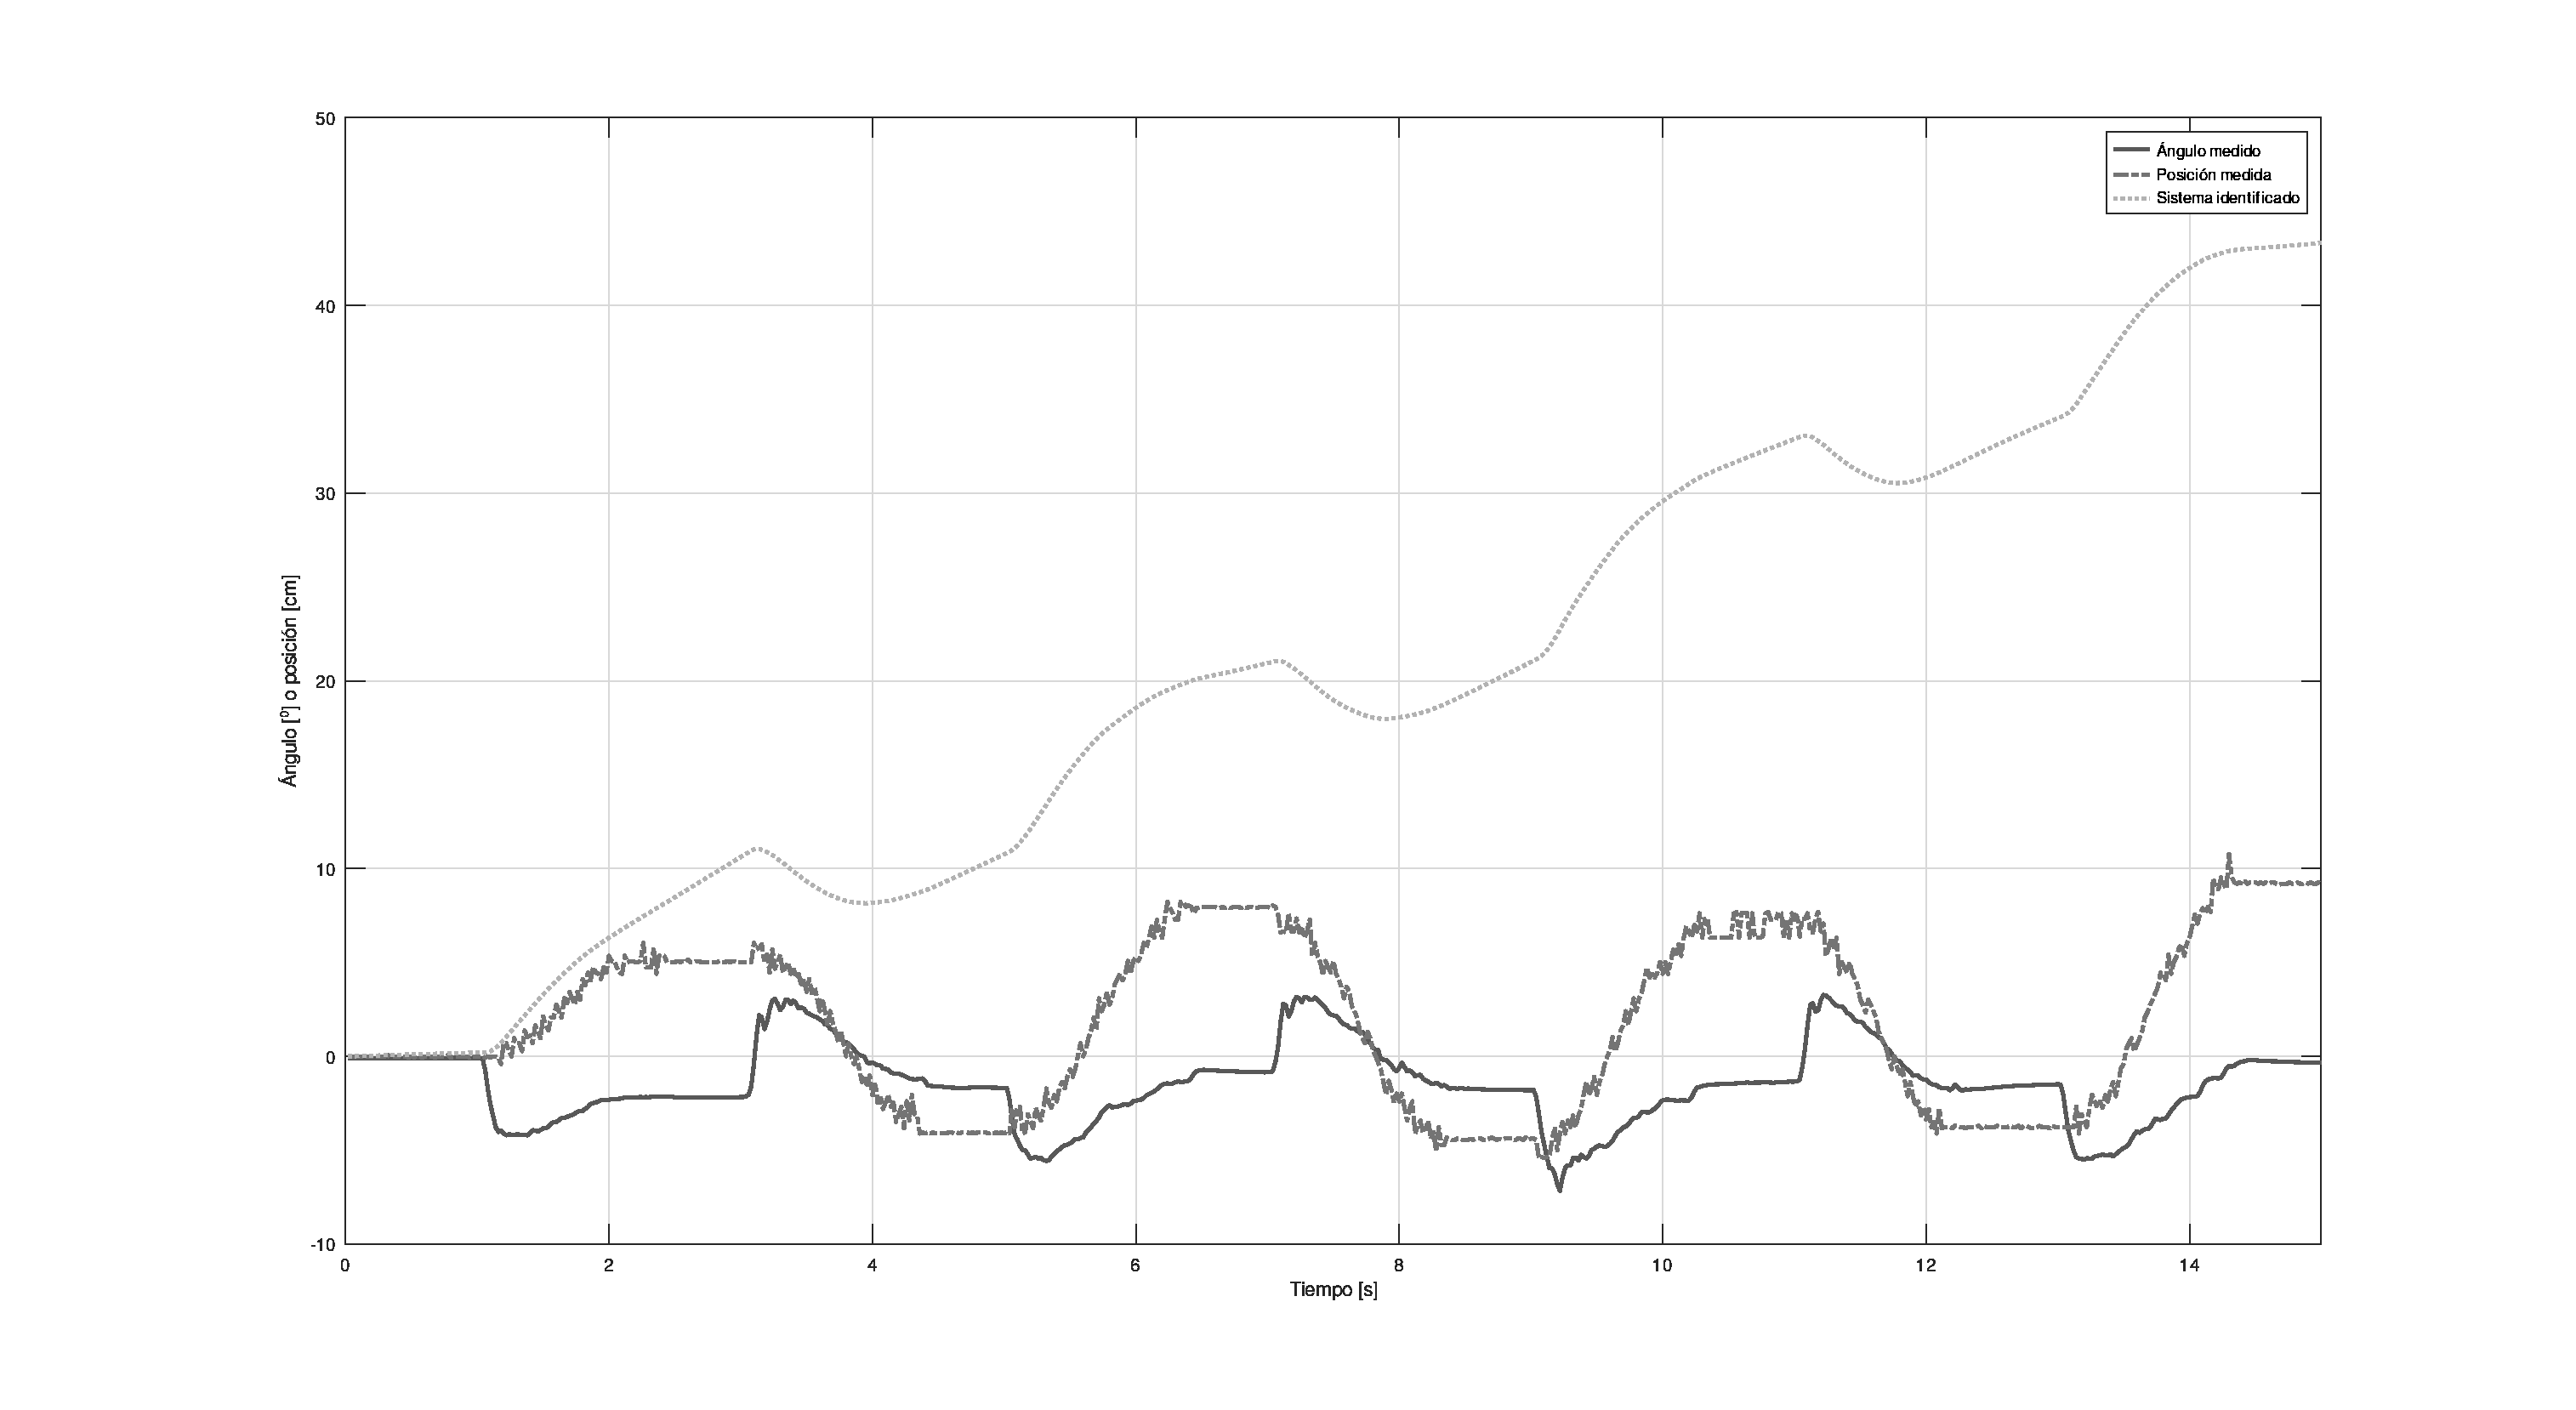
\includegraphics[width=\linewidth]{img/ident-carrito.eps}
    \caption{}
    \label{fig:ident-carro}
\end{figure}


% vim: ts=4 sts=4 sw=4 et lbr
